
An invariant property of a system is a property that is true about the
state of the sytem at all time instants.  In many cases, a
safety condition can be expressed as an invariance property.  For
example, if a set of states of a system are considered safe, then the
safety condition is the invariance property that the state of the
system at all time instants should belong to the safe set.  We
consider the problem of verifying {\it linear invariance} property of
discrete time affine hybrid systems.  A linear invariance property is
a linear constraint (inequality) that will be true for the
state of the system at every time instant.   To prove a linear
invariance property, it suffices to compute a positive invariant
containing the initial state and contained within the intersection of
sub-level set of linear inequalities.  Our approach is to compute an
augmented complex zonotope, which is a positive invariant and
satisfies the given linear constraints.  We derive a second order
conic program to compute the required augmented complex zonotope
positive invariant.

This chapter is organized as follows.  In the following section, we
discuss some of the related work on the problem of computing positive
invariants for affine hybrid systems.  We discuss the advantage of the
complex zonotope set representation in comparison to the other
approaches, which was discussed in more detail in the introductory
chapter.  In Section~\ref{sec:hybrid-system}, we define a discrete time affine
hybrid system.  In Section~\ref{sec:linear-invariance}, we define a linear invariance
property, positive invariant and show how we can verify linear
invariance by finding a positive invariant.  In Section~\ref{sec:verification-invariance}, we
discuss our procedure for verification of linear invariance based on
computing an augmented complex zonotope positive invariant.  We derive
a set of convex constraints, which are collectively equivalently to
second order conic constraint, compute the desired augmented complex
zonotope.  We also explain how to choose the template of the augmented
complex template, which is fixed apriori, while other parameters are
found by convex optimization.  In Sections~\ref{todo},~\ref{todo},
and~\ref{todo}, we discuss our experiments on three benchmark examples
that demonstrate the efficiency of our approach.

\section{Related Work}~\label{sec:invariance-related-work}
{\color{red} TODO}.  

\section{Discrete time affine hybrid system}~\label{sec:hybrid-system}
In a discrete time affine hybrid system, the state of the system is
specified by a discrete valued variable, called location, and a
continuous variable whose valuation is in the real Euclidean space of
a finite dimenstion.  The state of the system in each location has to
stay within a polyhedral set, called the staying condition.  The state
of the system can change by two kinds of transitions, {\it continuous
  transition} and {\it discrete transiton}.  In a continuous
transition, the discrete state of the system remains constant while
the continuous state changes by an affine transformation.  The affine
transformation has possible additive disturbance input, which is
bounded.  The parameters of the affine transformation of a continuous
transition depend on the location in which the transition takes place.
In a discrete transition, there is a change in the discrete variable
accompanied by an affine transformation of the continuous variable.
The transition is has precondition specified by a linear constraint,
called a guard, while the post-condition is the staying condition in
the location reached after transition.  A set of edges specifies
the possible discrete transitions, vis a vis, the locations between
which a discrete transition takes place, the parameters of the affine
transformation and the guard.   

{\it Sub-parallelotopic guards and staying conditions}: In this paper,
we consider hybrid systems where the guards and staying conditions can
be specified by a sub-parallelotope with a common template.  We note
that the class of sub-parallelotopic constraints are quite general and
can be used in the specification of many practical affine hybrid
systems.  

{\bf Model.}  We specify the discrete time affine hybrid system
by a tuple 
 %
\[
\system = \lt(\locations,\qtemp,\stay,\linmap,\inputset,\edgeset,\Psi\rt).
\]
%
The finite set of locations is $\locations$.  The sub-parallelotopic
template for specifying the guards and staying conditions is
$\qtemp\in\mat{k}{n}{\reals}$.  The staying set in a location
$\loc\in\locations$ is a sub-parallelotope
$\ptope{\qtemp}{\lsys{\stay_\loc}}{\usys{\stay_\loc}}$, whose pair of
lower and upper interval bounds is
$\stay_\loc=\lt(\lsys{\stay_\loc},\usys{\stay_\loc}\rt)$ .  The
parameters affine transformation in a location $\loc\in\locations$
consist of a linear transformation, specified by a matrix
$\linmap_\loc\in\mat{n}{n}{\reals}$, and a bounded additive
disturbance input set $\inputset_\loc\subset\reals^n$.  The set of
edges is $E$.  An edge $\edge\in\edgeset$ is specified by a tuple
%
\[
\edge=\lt(\edge_1,\edge_2,\usys{\edge},\lsys{\edge},\linmap_\edge,\inputset_\edge\rt).
\]
%
The before and after locations of a discrete transition along an edge
$\edge$ are $\edge_1,\edge_2$.  The guard on the transition along the
edge $\edge$ is the sub-parallelotope
$\ptope{\qtemp}{\lsys{\edge}}{\usys{\edge}}$, whose pair of
lower and upper interval bounds is
$\lt({\lsys{\edge}},{\usys{\edge}}\rt)$.
The parameters of the affine transformation for the discrete
transition along the edge $\edge$ consists of a linear map specified
by the matrix $\linmap_\edge\in\mat{n}{n}{\reals}$ and a bounded
additive disturbance input set $\inputset_\edge\subset\reals^n$.  The
set of initial states of the system is $\Psi\subseteq\locations\times\reals^n$.

{\bf Dynamics.}  A state of the hybrid system is a pair $(x,\loc)$,
where $x\in\reals^n$, called the {\it continuous state}, and
$\loc\in\locations$, called the {\it discrete state}.  A {\it
  trajectory} specifies the evolution of the state of the system as a
function of discrete time instants.  A trajectory is a function
$\maphtrj:\integers_{\geq 0}\ra\reals^n\times\locations$, such that
$\forall t\in\integers_{\geq 0}$, one of the following conditions is
true.
%
\begin{enumerate}
\item todo
\item todo
\end{enumerate}
%































{\color{red} TODO.}

\section{Linear invariance property}~\label{sec:linear-invariance}
A linear invariance property is a set of linear inequalities that are
satisfied by the state of the system at all time instants for every
trajectory starting in a given initial set.  Mathematically, it is
defined as follows.
%
\begin{definition}[Linear Invariance]
Let us consider a set of states
$\Psi\subseteq\reals^n\times\locations$, a real matrix 
${T\in\mat{r}{n}{\reals}}$ and a real vector $d\in\reals^r$.  We
say that \[\lt(\system,\Psi\rt)\models\invariance{T}{d}~~\text{(Linear invariance property)}~~\text{iff}\] 
%
\begin{align*}\
& \forall t\in\integers_{\geq 0},\forall
 x\in\bigcup_{q\in\locations}\lt(\reachset{t}{\Psi}\rt)_\loc:~~
 Tx\leq d.
\end{align*}
%
\end{definition}
%
To prove that a set of initial states satisfies a linear invariance
property, we can equivalently show the existence of a positive
invariant containing the initial states and satisfying the linear
constraints given in the property specification.  This is described below.
%
\begin{lemma}~\label{lem:pi-ver}
We have
$\lt(\system,\Psi\rt)\models\invariance{T}{d}$ iff there
exists a positive invariant $\Omega$ such that $\Psi\subseteq\Omega$
and $\forall \loc\in\locations~\forall x\in\Omega_{\loc}:~Tx\leq d$.
\end{lemma}
%
\begin{proof}
{\it Case 1:} Let us consider that there exists a positive invariant
$\Omega$ such that $\Psi\subseteq\Omega$ and $\forall
\loc\in\locations~\forall x\in\Omega_{\loc}:~Tx\leq d$.  Since
$\Omega$ is a positive invariant, we have
%
\[
\bigcup_{t\in\integers_{\geq 0}}\reachset{t}{\Omega}\subseteq\Omega
\]
%
\begin{align*}
  & \therefore\forall t\in\integers_{\geq 0}~\forall q\in\locations~\forall x\in\lt(\reachset{t}{\Omega}\rt)_\loc:~Tx\leq d\\
  & \%\%~~\text{since}~\Psi\subseteq\Omega\\
  & \forall t\in\integers_{\geq 0}~\forall q\in\locations~\forall x\in\lt(\reachset{t}{\Psi}\rt)_{\loc}:~Tx\leq d\\
  & \lt(\Psi,\system\rt)\models\invariance{T}{d}.
\end{align*}
%
{\it Case 2:}  Let us consider that $\lt(\system,\Psi\rt)\models\invariance{T}{d}$.  Let us denote 
%
\[
\Omega=\bigcup_{t=0}^\infty\reachset{t}{\Psi}.
\]
% 
Then by Lemma~\ref{lem:exact-pi}, $\Omega$ is a positive invariant.  By
the definition of linear invariant property, we get 
%
\begin{align*}
& \forall t\in\integers_{\geq 0},\forall
 x\in\bigcup_{q\in\locations}\lt(\reachset{t}{\Psi}\rt)_\loc:~~
 Tx\leq d\\
 & \equivalent \forall q\in\locations~\forall
x\in\lt(\bigcup_{t=0}^\infty\reachset{t}{\Psi}\rt)_\loc:~~Tx\leq d\\
 & \equivalent \forall q\in\locations~\forall
x\in\Omega_\loc:~~Tx\leq d.
\end{align*}
%
The lemma follows from the results in both the above cases.
\end{proof}
%


\section{Verification using complex zonotope}~\label{sec:verification-invariance}
{\color{red} TODO}.

\section{Experiments}
\subsection{Robot with a saturated controller}
Our first example is a veriication problem for the model of a
self-balancing two wheeled robot called
NXTway-GS1\footnote{\url{http://www.mathworks.com/matlabcentral/fileexchange/19147-nxtway-gs-self-balancing-two-wheeled-robot-controller-design}}
by Yorihisa Yamamoto, which was presented in the ARCH
workshop~\cite{heinz2014benchmark}. We consider the linearized sampled
data (discrete time) networked control system model from the paper.
The state of the plant is represented by a 6-dimensional vector
$x_p=(\dot{\theta},\theta,\dot{\psi},\psi,\dot{\phi},\phi)^T$, where
$\theta$ is the average angle of the left and right wheel, $\psi$ is
the body pitch angle, $\phi$ is the body yaw angle, and the rest
coordinates are their respective angular velocities.  The output of
the plant is represented by a 3-dimensional vector
$\lt(\dot{\psi}_{\operatorname*{out}},\theta_{m_1},\theta_{m_r}\rt)^T$
such that $y_p=C_px_p$.  The input to the plant is a two dimensional
vector $u_p$.  The dynamics of the plant is given by the differential
equation $\dot{x}_p=A_px_p+B_pu_p$.  In the sampled data system, the
state of the plant is sampled every 4s.

The controller state is represented by a 6-dimensional vector $x_c$,
and the input to the controller is denoted
$u_c=\lt({u^\pr}_c,u^\dpr_c\rt)$.  The controller inputs
${{u^\pr}_c}$ and $u^\dpr_c$ are both 2-dimensional inputs.  The input
$u^\dpr$ is an uncertain input which is in the range $[-100,100]$.  The
controller dynamics is given by the equations
%
\begin{align*}
  & \dot{\tau}=1,~~\tau(4^+)=0\\
  & {u^\pr}_c(\tau)=\hat{u}_c(0)~\text{if}~\tau\in[0,4)\\
  & {u^\pr}_c(4)=y_p(\tau)\\
  & \dot{x_c}(\tau)={A}_cx_c(\tau)+{B}_cu_c(\tau)\\
  & y_c(\tau)=C_cx_c(\tau)+D_cu_c(\tau).
\end{align*}
%
The controller has a 2-dimensional output $y_c$ which is processed to
provide input to the plant.  The processor has a saturation limit on
the output received from the controller.  The saturated controller
output is given by the equation
%
\begin{align*}
u_p=D_p\lt(\join{\lt(\meet{y_c}{\mymatrix{v\\v}}\rt)}{\mymatrix{-v\\-v}}\rt).~\numberthis\label{eqn:sat1}
\end{align*}
%
where $v=100$ is a saturation limit.  The sampled data dynamics with
saturation can be modeled by an affine discrete time hybrid system,
where the switching is controlled by relevant guards on $u_p$.
However, if we consider the continuous state of the affine hybrid
system as $\lt(x_p,x_c,u_p\rt)^T$, we observed that some of the
directions are unbounded.  Therefore, we decoupled some unbounded
directions of the dynamics from the bounded directions by making
appropriate linear transformation of the coordinates.  The linear
transformation is composed by two transformations, one of which
involved Jordan decomposition in Matlab.

\begin{table}
{\scriptsize
\begin{align*}
& F_1  = \lt[\begin{matrix}
3.6929   &      0  &  0.7302  &  7.9715 &  14.5019 &   -0.0072 &
0.0720 &   -2.7354\\
    3.6929   &      0  &  0.7302  &  7.9715 &  14.5019 &  -0.0072  &  0.0720  & -2.7354\\
    0.9562    &     0  &  0.0019 &  -0.0021 &  -0.0022 &   -0.0000 &  -0.0001 &  -0.0002\\
         0 &   0.6910    &     0    &     0  &       0     &    0   &      0    &     0\\
    0.8833     &    0  & -0.1154 &  -1.2943 &  -2.3520  &  0.0012 &  -0.0118  &  0.4427\\
   -0.4712    &     0 &  -0.0812 &    0.1151  & -1.4845  &  0.0007 &  -0.0071  &  0.2819\\
   -0.1560     &    0 &  -0.0459 &  -0.3173  &  0.3650  &  0.0003  & -0.0023  &  0.1162\\
   -0.7719   &      0 &  -0.1248  & -1.4264 &  -2.5901  &  0.9973 &  -0.0131  &  0.4869\\
   -0.7544  &       0  & -0.1243 &  -1.4204 &  -2.5792  &  0.0013 &   0.9825 &   0.4796\\
   -0.1905   &      0  & -0.0148  & -0.2081 &  -0.3751  &  0.0002  &  0.0033  &  1.0651
\end{matrix}\rt]\\
& F_2 = \lt[\begin{matrix}
0.2543  &  0.2543\\
    0.2543  &  0.2543\\
   -0.0001 &  -0.0001\\
         0 &        0\\
   -0.0413 &  -0.0413\\
    0.0219  &  0.0219\\
    0.0102 &   0.0102\\
    0.0431 &   0.0431\\
    0.0428 &   0.0428\\
    0.0065 &   0.0065\\
\end{matrix}\rt],
~F_3 = 10^{-2}\times\lt[\begin{matrix}
 0.0000    &     0  & -0.0330 &   2.0218\\
    0   &      0  & -0.0330 &  -2.0218\\
    0  &       0 &   -0  &  0\\
   -0  &       0  &  0 &   0.0109\\
   -0.0118 &        0  &  0.0172  &  0 \\
    0.0436  &       0 &   0.0003 &  0 \\
   -0.0478   &      0  &  0.0034 &   0 \\
  -13.3924 &        0 &   0.0062 &   0 \\
    0.0909     &    0  &  0.0061 &  0\\
   -0.0798  &       0 &   0.0017  &  0\\
\end{matrix}\rt]
\end{align*}}
\caption{Matrices of the transformed system dynamics}~\label{tab:matrices-nxt}
\end{table}


After decomposition, the bounded dynamics with saturation could be
modeled in a 10-dimensional state space, which is described below.
%
\begin{align*}
\mymatrix{x(t+1)\\y(t+1)}=F_1\trj{x}{t}+F_2sat\lt(\trj{y}{t}\rt)+F_3\trj{u}{t},
\end{align*}
where $\trj{x}{t}\in\realset^8$ is the transformed state of the
composite system of plant and controller, $\trj{y}{t}\in\realset^2$ is
the input sent by the controller, $\trj{u}{t}\in\lt[-100,100\rt]^4$ is
the bounded additive disturbance input and $\operatorname*{sat}$ is
the saturation function which limits the controller input received by
the plant.  The body pitch angle is the first co-ordinate, i.e.,
$\psi=x_1$.  The matrices $F_1$, $F_2$ and $F_3$ are given in
Table~\ref{tab:matrices-nxt}.  The matrices for the original
(untransformed system) are given in the appendix.  The saturation
function is defined as follows.  The saturation function is given as
follows.
%
\begin{align*}
& \text{If
  saturated}~~\operatorname*{sat}\lt(y_i\rt) = max\lt(-\delta
 d_p,min\lt(y_i,\delta d_p\rt)\rt),~\forall i\in\{1,2\},\\
&\text{If unsaturated}~~ sat\lt(y_i\rt)=y_i~\forall i\in\{1,2\}.
\end{align*}
%
where $\delta=100$ and $d_p=0.0807$.  
%
{\color{red} TODO Input figure here}.

{\bf Model complexity:} The 2-dimensional input $y$ on which the
positive and negative saturation is defined can thus be divided into 9
different regions, where the system exhibits different dynamics.  We
model each of the discrete time dynamics by a self edge on a common location.
Therefore, the saturated model consists of a single location with 9
self-edges having appropriate linear guards and transition matrices.
On the other hand, the unsaturated model is a linear system having
uncertain input, which is therefore modeled by only one location.

\emph{Size of saturated model}: 10 dimensional, 1 location and 9 edges.

\emph{Size of unsaturated model}: 10 dimensional, 1 location, 0 edges.

{\bf Linear invariance property to verify}: The safety requirement is
that the \emph{body pitch angle} of the robot, which in our model is
denoted by $x_1$, should be bounded within some value. In the
benchmark, it was suggested that for the saturated system
$x_1\in\lt[-\frac{\pi}{2}+\epsilon,\frac{\pi}{2}-\epsilon\rt]:~\epsilon>0$,
while $x_1\in\lt[\frac{-\pi}{2.26},~\frac{\pi}{2.26}\rt]$ for the
unsaturated system. The initial set is the origin.  Therefore, we want
to find a small bound $d$ on the valued of
$\absolute{\psi}=\absolute{x_1}$.  As the model is symmetric, it is
sufficient to find a bound along the positive direction.  Therefore,
we have to find a small enough $d$ such that $\lt(T,d\rt)$, where
$T=\mymatrix{1&\repmat{0}{1}{9}}$, is a linear invariance property.

{\bf Experiment settings.}

\emph{Augmented complex zonotope: }  The primary template for the hybrid system
is chosen as the collection of the (complex) eigenvectors of linear
matrices of all affine maps for the edge transitions, the orthonormal
vectors to the guarding hyperplane normals and the projections of the
eigenvectors on the subspace spanned by the orthonormal vectors.  For
the linear system, it consists of the eigenvectors of the linear map,
the input set template and its multiplication by the linear matrix
(related to affine map) and square of the linear matrix.

\emph{SpaceEx:      } Concerning
the experiment using SpaceEx, we tested with the octagon template and
a template with $400$ uniformly sampled support vectors distributed
uniformly in space.  
\begin{table}
\begin{minipage}{1\textwidth}
\centering
\begin{tabular}{|l|c|c|c|}
\hline
\multicolumn{2}{|c|}{\multirow{2}{*}{Method}} &
\multirow{2}{*}{Bound on pitch angle} & \multirow{2}{*}{Comp. time (s)}\\
\multicolumn{2}{|c|}{} & & \\
\hline
\multirow{4}{*}{SpaceEx} & octagon & \multirow{2}{*}{$>1000$} &
\multirow{2}{*}{Not terminate in $<180s$}\\
& template & & \\
\cline{2-4}
& 400 support & \multirow{2}{*}{UB} & \multirow{2}{*}{Not terminate in
  $<180s$}\\
& vectors & &\\
\hline
\multicolumn{2}{|c|}{\multirow{2}{*}{Suggested in~\cite{heinz2014benchmark}}} &
\multirow{2}{*}{$1.39$} & \multirow{2}{*}{n/a}\\
\multicolumn{2}{|c|}{} & &\\
\hline
\multicolumn{2}{|c|}{\multirow{2}{*}{Augmented complex zonotope}} & \multirow{2}{*}{$1.29$} &
\multirow{2}{*}{$4$}\\
\multicolumn{2}{|c|}{} & & \\
\hline
\end{tabular}
\caption{Unsaturated robot model: results}
~\label{tab:robot-unsaturated}
\end{minipage}
\hspace{0em}
\begin{minipage}{1\textwidth}
\centering
\begin{tabular}{|l|c|c|c|}
\hline
\multicolumn{2}{|c|}{\multirow{2}{*}{Method}} &
\multirow{2}{*}{Bound on pitch angle} & \multirow{2}{*}{Comp. time (s)}\\
\multicolumn{2}{|c|}{} & & \\
\hline
\multirow{4}{*}{SpaceEx} & octagon & \multirow{2}{*}{$>1000$} &
\multirow{2}{*}{Not terminate in $<180s$}\\
& template & & \\
\cline{2-4}
& 400 support & \multirow{2}{*}{UB} & \multirow{2}{*}{Not terminate $<180s$}\\
& vectors & & \\
\hline
\multicolumn{2}{|c|}{\multirow{2}{*}{Suggested in~\cite{heinz2014benchmark}}} &
\multirow{2}{*}{$1.571-\epsilon:~\epsilon>0$} & \multirow{2}{*}{n/a}\\
\multicolumn{2}{|c|}{} &  &\\
\hline
\multicolumn{2}{|c|}{\multirow{2}{*}{Augmented complex zonotope}} & \multirow{2}{*}{$1.16$} &
\multirow{2}{*}{45}\\
\multicolumn{2}{|c|}{} & &\\
\hline
\end{tabular}
\caption{Saturated robot model: results}
~\label{tab:robot-saturated}
\end{minipage}
\end{table}


\tbf{Results.}  For both the hybrid and the linear systems, we could
verify smaller magnitudes for the bounds on the pitch angle than what
is proposed in the benchmark~\cite{heinz2014benchmark}.  But the
SpaceEx tool could not find a finite bound for either of the above
systems.  The results are reported in the
Tables~\ref{tab:robot-unsaturated} and~\ref{tab:robot-saturated}.

\tbf{Remark.}  We have discussed in the review of polytopes that
although a linear system has a polytopic invariant, computing it can
be difficult.  The representation size of a polytopic invariant for a
fixed dimension can be arbitrarily large.  In our unsaturated model
which is linear, some of the eigenvalues are complex and their
magnitudes are close to one.  Possibly this is the reason SpaceEx
could not find an invariant even with 400 support vectors distributed 
uniformly in space.  But in our approach, since we use the complex
eigen-structure, we could find the desired invariant for the
unsaturated (linear) model.  Furthermore, we we also computed the
invariant for the saturated (hybrid) model.



\subsection{Networked platoon of vehicles}
Our third example is a model of a networked cooperative platoon of
vehicles, which is presented as a benchmark in the ARCH
workshop~\cite{makhlouf2014networked}.  The platoon consists of three
vehicles $M_1$, $M_2$ and $M_3$ along with a leader board ahead $M_4$.
The movement of the vehicles is dependent on the communication between
them their relative distances, velocities and accelerations.  The
distance between a vehicle $M_i$ and its next
vehicle $M_{i+1}$, relative to a reference distances $d_i^{ref}$ is
denoted $e_i$.  The acceleration of the leader vehicle is $a_L$ which
ranges between $[-9,1]m/s$.  The state of the system is denoted
by a vector
$x=\lt[e_1,\dot{e}_1,\ddot{e}_1,e_2,\dot{e}_2,\ddot{e}_2,e_3,\dot{e}_3,\ddot{e}_3\rt]$.
The dynamics of the platoon is different in the two cases when there
is full communication and when there is total failure of
communication.  These dynamics are described by differential equations,
%
\begin{align*}
& \dot{x}=A_cx+B_ca_L~\text{when there is communication}\\
& \dot{x}=A_nx+B_na_L~\text{when there is failure of communication}.
\end{align*}
%
where the pairs of matrices $(A_c,B_c)$ and $(A_n,B_n)$ are different.
In any given mode, the
dynamics of the system is exponentially stable.  So, the lyapunov
exponent (measure of stability) is higher in case of slow switching
than fast switching.  Therefore, in our evaluation of this example, we
also consider a model having integer switching times, which is less
stable.
%
\begin{figure}
\center
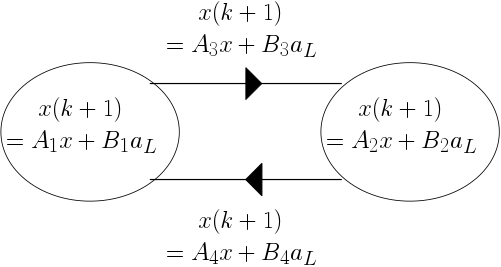
\includegraphics[scale=0.5]{fig/platton-dynamics.png}
\caption{Time discretized model of networked platoon}~\label{fig:model-platoon}
\end{figure}
%
%
\begin{table}
\caption{Matrices for discrete time slow switching model}~\label{matrices:slow}
{\scriptsize
$A_1=\mymatrix{0.2766  &  0.2855&   -0.0235&    0.2550&    0.2352&   -0.0429&    0.1245&    0.0956&   -0.0234\\
   -0.0917&   -0.0848&    0.0392&   -0.0517&    0.0134&    0.0023&    0.0003&    0.0385 &  -0.0166\\
   -0.0531&   -0.0485&    0.0404&    0.0434&    0.0807&   -0.0172&    0.0301&    0.0363&   -0.0097\\
    0.1406&    0.1632&    0.0002&    0.0313&    0.1166&   -0.0122&    0.1017&    0.1309&   -0.0431\\
   -0.0411&   -0.0589&   -0.0421&   -0.0512&   -0.1530&    0.0575&   -0.0476&   -0.0321&    0.0051\\
   -0.0393&   -0.0402&   -0.0111&   -0.0641&   -0.0754&    0.0467&    0.0497&    0.0760&   -0.0251\\
    0.0628&    0.0763&    0.0095&    0.0634&    0.0987&    0.0081&   -0.0788&    0.0489&   -0.0436\\
   -0.0088&   -0.0158&   -0.0081&   -0.0351&   -0.0452&   -0.0726&   -0.0621&   -0.2082&    0.0863\\
   -0.0246&   -0.0235&   -0.0078&   -0.0572&   -0.0547&   -0.0183&   -0.1049&   -0.1146&    0.0307}$
$A_2=\mymatrix{ 0.2398 &   0.2204&   -0.0715&   -0.0000&    0.0000&   -0.0000&   -0.0000&    0.0000&   -0.0000\\
   -0.1148&   -0.1083&    0.0352&   -0.0000&   -0.0000&    0.0000&   -0.0000&   -0.0000&    0.0000\\
   -0.0565&   -0.0567&    0.0176&   -0.0000&   -0.0000&   -0.0000&   -0.0000&   -0.0000&    0.0000\\
    0.0178&    0.5068 &  -0.0658&    0.2410&    0.3042&   -0.1113&   -0.0000&    0.0000&   -0.0000\\
   -0.1056&  -0.3026&    0.0327&   -0.1329&   -0.1627&    0.05657&   -0.0000&   -0.0000&    0.0000\\
   -0.1089&   -0.1100&   -0.0055&   -0.0675&   -0.0720&    0.0204&   -0.0000&   -0.0000&    0.0000\\
    0.2386&   -0.0802&    0.0965&    0.1118&    0.1544&    0.0604&    0.1197&    0.2679&   -0.1103\\
    0.0762&    0.3143&   -0.0998&   -0.0213&   -0.0283&   -0.0726&   -0.1404&   -0.2191&    0.0779\\
   -0.0043&    0.0212&   -0.0122&   -0.0468&   -0.0413&   -0.0171&   -0.0991&   -0.0990&    0.0251}$
 $B_1=\mymatrix{1.8593\\
    0.2855\\
    1.0848\\
    0.5394\\
    0.1632\\
    1.1437\\
    0.1950\\
    0.0763\\
    1.1596}$
$B_2=\mymatrix{1.7651\\
    0.2204\\
    1.1083\\
    2.1977\\
    0.5068\\
    1.4109\\
   -1.2748\\
   -0.0802\\
    1.0966}$
$B_3=\mymatrix{2.8411\\
    0.0019\\
    1.0006\\
    0.9508\\
    0.0007\\
    1.0009\\
    0.3775\\
    0.0003\\
    1.0009}$    
$B_4=\mymatrix{2.2276\\
    0.0001\\
    1.0001\\
    2.7152\\
   -0.0005\\
    1.0000\\
   -0.4469\\
    0.0001\\
    1.0000\\
}$
~~$A_3=A_4=\repmat{0}{9}{9}$.
}
\end{table}
%
\begin{table}
\caption{Matrices for discrete time fast switching model}~\label{matrices:fast}
{\scriptsize
$A_1=A_3=\mymatrix{ 0.8902 &   0.6370&   -0.1484&    0.0588&   -0.0050&    0.0001&    0.0157&   -0.0148&    0.0059\\
   -0.2340&    0.1889&   -0.1119&    0.1267&    0.0147&   -0.0039&    0.0363&   -0.0201&    0.0104\\
    0.1755&    0.7560&   -0.2251&   -0.0959&   -0.0989&    0.0181&   -0.0373&   -0.0273&    0.0018\\
    0.0462&    0.0643&    0.1514&    0.8509&    0.7076&   -0.1685&    0.0303&    0.0218&   -0.0038\\
    0.0934&    0.1271&    0.1151&   -0.3284&    0.2923&   -0.1466&    0.0660&    0.0517&   -0.0108\\
    0.1262&    0.6998&    0.0092&    0.1826&    0.7469&   -0.2119&   -0.0885&   -0.0830&    0.0189\\
    0.0116&    0.0170&    0.0026&    0.0241&    0.0282&    0.1719&    0.8532&    0.7238&   -0.1801\\
    0.0256&    0.0364&    0.0064&    0.0505&    0.0619&    0.1543&   -0.3320&    0.3231&   -0.1730\\
    0.1047&    0.6724&    0.0017&    0.1502&    0.6976&    0.0119&    0.2247&    0.7581&   -0.1875}$
$A_2=A_4=\mymatrix{0.8898 &   0.6325&   -0.1463&    0.0000&    0.0000&    0.0000&    0.0000&    0.0000&   -0.0000\\
   -0.2348&    0.1775&   -0.1094&    0.0000&    0.0000&    0.0000&    0.0000&    0.0000&   -0.0000\\
    0.1756&    0.7674&   -0.2136&    0.0000&    0.0000&    0.0000&    0.0000&    0.0000&   -0.0000\\
    0.0939&    0.3146&    0.1064&    0.9098&    0.6995&   -0.1686&    0.0000&    0.0000&   -0.0000\\
    0.1708&    0.6120&    0.0043&   -0.2012&    0.2985&   -0.1533&    0.0000&    0.0000&   -0.0000\\
    0.1687&    0.5757&    0.1151&    0.1829&    0.7569&   -0.1980&    0.0000&    0.0000&   -0.0000\\
   -0.0364&   -0.2331&    0.0460&    0.0254&    0.0312&    0.1721&    0.9004&    0.7304&   -0.1778\\
   -0.0529&   -0.4476&    0.1169&    0.0548&    0.0704&    0.1571&   -0.2263&    0.3541&   -0.1728\\
    0.1044&    0.6771&   -0.0016&    0.1418&    0.6953&    0.0121&    0.2199&    0.7571&   -0.1877}$    
$B_1=B_3=\mymatrix{0.3930\\
    0.6370\\
    0.8111\\
    0.0200\\
    0.0643\\
    0.6840\\
    0.0051\\
    0.0170\\
    0.6476\\
}$
$B_2=B_4=\mymatrix{0.3918\\
    0.6325\\
    0.8225\\
    0.0979\\
    0.3146\\
    0.2105\\
   -0.0727\\
   -0.2331\\
    0.6581}$
}
\end{table}
%

{\bf Time discretized models: } We could discretized the dynamics of
both models with large minimum switching time and integer switching
time.  The time discretized model has 2 locations and 4 edges, as
described in Figure~\ref{fig:model-platoon}.  The continuous state is
9-dimensional.  The matrices denoted in the figure are different for
the case of slow switching and fast switching and are given in
Tables~\ref{matrices:slow} and~\ref{matrices:fast}, respectively.


{\bf Linear invariance property: } The verification challenge proposed
in~\cite{makhlouf2014networked} is to find the minimum possible
reference distances $d_i^{ref}~\forall i\in\set{1,2,3}$, such that the
vehicles do not collide.  Any set of upper bounds on $-e_1$, $-e_2$,
and $-e_3$ are safe lower limits on the respective reference
distances.  We express the verification problem in terms of three
linear invariance properties, as follows.  For each ${T_i:~1\leq i\leq
3}$, where
%
$ T_1=\mymatrix{-1 & \repmat{0}{1}{8}},~
T_2=\mymatrix{\repmat{0}{1}{3} & -1 &\repmat{0}{5}{3}}$ and
 ${T_3=\mymatrix{\repmat{0}{1}{6}& -1 &\repmat{0}{2}{3}}},
$
%
find an upper bound on each $d_i:~i\in\set{1,2,3}$ such that
$\lt(T_i,d_i\rt)$ is a linear invariance property of the system.

\tbf{Experiment settings.}  We chose the primary template
as the collection of the (complex) eigenvectors of linear matrices of
the affine maps in the the two locations and their binary products,
the axis aligned box template and the templates used for
overapproximating the input sets. For the SpaceEx tool, we
experimented with two templates, octagon and hundred uniformly sampled
support vectors.

\tbf{Results.}  For the large minimum dwell time of $20s$, the
discrete time SpaceEx implementation and also a method based on using
real zonotopes~\cite{makhlouf2014networked} could verify slightly
smaller bounds compared to our approach.  But for the small minimum
dwell time ($1s$) model, SpaceEx could not even find a finite set of
bounds, whereas our approach could verify a finite set of bounds.  The
reason is that the fast system model is more stable compared to the
slow switching.  Possibly because complex zonotope captures
contraction along complex eigenvectors, we could find a finite
invariant for even the less stable fast switching model.  These
results are reported in the Tables~\ref{tab:largedwell-platoon}
and~\ref{tab:largedwell-platoon1}.
%

\begin{table}
\begin{tabular}{|l|c|c|c|c|c|}
\hline
\multicolumn{2}{|c|}{\multirow{4}{*}{Method}} & \multicolumn{4}{|c|}{\multirow{2}{*}{Slow switching}}\\
\multicolumn{2}{|c|}{} & \multicolumn{4}{|c|}{}\\
\cline{3-6}
\multicolumn{2}{|c|}{} & \multirow{2}{*}{$-e_1\leq$} & \multirow{2}{*}{$-e_2\leq$} & \multirow{2}{*}{$-e_3\leq$} & Comp.\\
\multicolumn{2}{|c|}{} & & & & time (s)\\
\hline
\multirow{4}{*}{SpaceEx} & octagon & \multirow{2}{*}{28} &
\multirow{2}{*}{27} & \multirow{2}{*}{10}& \multirow{2}{*}{$>180s$}\\
& template & & & &\\
\cline{2-6}
& 100 support & \multirow{2}{*}{28} & \multirow{2}{*}{25} &
\multirow{2}{*}{13} & \multirow{2}{*}{1.3}\\
& vectors & & & &\\
\hline
\multicolumn{2}{|c|}{\multirow{2}{*}{Real zonotope~\cite{makhlouf2014networked}}} &
\multirow{2}{*}{25} & \multirow{2}{*}{25} & \multirow{2}{*}{10} & \multirow{2}{*}{n/a}\\
\multicolumn{2}{|c|}{} & & & &\\
\hline
\multicolumn{2}{|c|}{\multirow{2}{*}{Augmented complex zonotope}} &
\multirow{2}{*}{28} & \multirow{2}{*}{26} &
\multirow{2}{*}{12} & \multirow{2}{*}{12}\\
\multicolumn{2}{|c|}{} & & & & \\
\hline
\end{tabular}
\caption{Experimental results: Slow switching networked platoon}~\label{tab:largedwell-platoon}

%% %
%% \end{table}
%% %
%% \begin{table}
{\vspace{2em}
\begin{tabular}{|l|c|c|c|c|c|}
\hline
\multicolumn{2}{|c|}{\multirow{4}{*}{Method}} & \multicolumn{4}{|c|}{\multirow{2}{*}{Fast switching}}\\
\multicolumn{2}{|c|}{} & \multicolumn{4}{|c|}{}\\
\cline{3-6}
\multicolumn{2}{|c|}{} & \multirow{2}{*}{$-e_1\leq$} & \multirow{2}{*}{$-e_2\leq$} & \multirow{2}{*}{$-e_3\leq$} & Comp.\\
\multicolumn{2}{|c|}{} & & & & time (s)\\
\hline
\multirow{4}{*}{SpaceEx} & octagon & \multirow{2}{*}{$>1000$} &
\multirow{2}{*}{$>1000$} & \multirow{2}{*}{$>1000$} &
\multirow{2}{*}{$>180s$}\\
& template & & & &\\
\cline{2-6}
& 100 support & \multirow{2}{*}{$>1000$} & \multirow{2}{*}{$>1000$} &
\multirow{2}{*}{$>1000$} & \multirow{2}{*}{$>180s$}\\
& vectors & & & & \\
\hline
\multicolumn{2}{|c|}{\multirow{2}{*}{Augmented complex zonotope}} &
\multirow{2}{*}{46} & \multirow{2}{*}{54} &
\multirow{2}{*}{57} & \multirow{2}{*}{12.6}\\
\multicolumn{2}{|c|}{} & & & & \\
\hline
\end{tabular}
%
\caption{Experimental results: Fast switching networked Platoon}~\label{tab:largedwell-platoon1}
}
\end{table}



\subsection{Perturbed double integrator}
Our second example is a perturbed double integrator system given
in~\cite{rakovic2004computation}.  The closed loop system with a
feedback control is piecewise affine, having four different affine
dynamics in four different regions of space, as
%
\begin{align*}~\label{eqn:pwa-regions}
& \trj{x}{t+1}=M_i\trj{x}{t}+w.~~~
 i=\left\{\begin{array}{l}
1,~\text{if}~x_1\geq 0~\text{and}~x_2\geq 0\\
2,~\text{if}~x_1\leq 0~\text{and}~x_2\leq 0\\
3,~\text{if}~x_1\leq 0~\text{and}~x_2\geq 0\\
4,~\text{if}~x_1\geq 0~\text{and}~x_2\leq 0\\
\end{array} \rt.,\\
&~M_1=M_2=\lt[\begin{matrix}
0.4103  &  0.0653\\
  -0.2949  &  0.5327
\end{matrix}\rt],~M_3=M_4=\lt[\begin{matrix}
0.4103  &  -0.0653\\
  0.2949  &  0.5327
\end{matrix}\rt].
\end{align*}

The additive disturbance input $w$ is bounded as $\|w\|_{\infty}\leq
0.2$.  

We perform two different experiments on this system.  In the first
experiment, we try to verify the smallest possible magnitude of bounds
on the two coordinates, denoted $x_1$ and $x_2$. We compare these
bounds with that found by the SpaceEx tool.  In the second experiment,
we try to quickly compute a large invariant for the system under the
safety constraints given in~\cite{rakovic2004computation}.  The given
safety constraints are $\|x\|_{\infty}\leq 5$.  In the latter case, we
maximize the sum of the scaling factors and differences of the upper
and lower interval bounds of the augmented complex zonotopic
invaraint.  Furthermore, we decompose the given safety constraints as
the intersection of four different sets of safety constraints.  For
each set of safety constraints, we compute a large augmented complex
zonotopic invariant.  Then the desired invariant is the intersection
of four augmented complex zonotopic invariants.  Although we may not
find the largest possible (maximal) invariant by this approach, still
the optimizer will try to maximize the size of the invariant.  We draw
comparison in terms of the computation time with the reported result
for the MPT tool~\cite{rakovic2004computation}.

In our formalism, we model the system with $4$ locations and $12$
edges connecting all the locations.  Appropriate staying conditions
are specified in each location, reflecting the division of the state
space into different regions where the dynamics is affine. The initial
set is the origin. The same model is specified in SpaceEx.

\tbf{Size of model}: 2 dimensions, 4 locations and 12 edges.

\tbf{Experiment settings}.  For the primary template, we collected the
(complex) eigenvectors of all linear matrices of the affine maps and
their binary products. For the SpaceEx tool, we experimented with two
different templates, the octagon template and a template with 100
uniformly sampled support vectors.

\tbf{Results.}  In the first experiment, we verified sligtly smaller bounds
for $x_1$ than that of SpaceEx, while the bounds verified for $x_2$
were equal for both methods.  In our second experiment on this
example, the computation time for finding a large invariant by our
method is significantly smaller than that of the reported result for
the MPT tool.  The results are summarized in the
Tables~\ref{tab:smallinv-pdi} and~\ref{tab:largeinv-pdi}.

\begin{table}
\center
\begin{tabular}{|l|c|c|c|c|}
\hline
\multicolumn{2}{|c|}{\multirow{2}{*}{Method}} &
\multirow{2}{*}{$\lt|x_1\rt|\leq$} & \multirow{2}{*}{$\lt|x_2\rt|\leq$} & Comp.\\
\multicolumn{2}{|c|}{} & & & time (s) \\
\hline
\multirow{4}{*}{SpaceEx} & octagon & \multirow{2}{*}{0.38} &
\multirow{2}{*}{0.43} & \multirow{2}{*}{1.7}\\
& template & & &\\
\cline{2-5}
& 100 support & \multirow{2}{*}{0.38} & \multirow{2}{*}{0.43} & \multirow{2}{*}{23.6}\\
& vectors & & &\\
\hline
\multicolumn{2}{|c|}{\multirow{2}{*}{ACZ invariant}} &
\multirow{2}{*}{0.37} & \multirow{2}{*}{0.43} & 
\multirow{2}{*}{5.1}\\
\multicolumn{2}{|c|}{} & & &\\
\hline
\end{tabular}
\caption{Small invariant computation: Perturbed double
  integrator}
~\label{tab:smallinv-pdi}
\end{table}
%
\begin{table}
\center
\begin{tabular}{|c|c|}
\hline
\multirow{2}{*}{Method} & Comp.\\
& time (s)\\
\hline
\multirow{2}{*}{MPT tool~\cite{rakovic2004computation}} & \multirow{2}{*}{107}\\
& \\
\hline
\multirow{2}{*}{ACZ} & \multirow{2}{*}{12}\\
& \\
\hline
\end{tabular}
\caption{Large invariant computation: Perturbed double integrator}
~\label{tab:largeinv-pdi}
\end{table}
%% \tbf{Remark.}  The overapproximation quality of SpaceEx reduces when
%% there are large number of edges, because then in each step, a union of
%% many different polytopes has to be overapproximated using support
%% vectors.  In contrast, our approach uses optimization to learn an
%% appropriate invariant, avoiding the union operations.  Possibly
%% because of this reason, we verified smaller bounds than SpaceEx on
%% this example.




